% Work-MAT -- 2. rocnik, hodina 06. Vetev kvadraticke funkce a kontrola slozenim.
\documentclass[11pt,a4paper]{article}
\input{../../sablony/pripravy/priprava.sty}
\usepackage{tikz}
\usetikzlibrary{arrows.meta}
\nastavPripravu{2. ročník}{Inverzní funkce}{06}{Inverzní funkce IV: omezení oboru}
\begin{document}
\poznamka{Didaktické těžiště: prostota závisí i na definičním oboru, nejen na algebraickém předpisu. Orientačně 5 min opakování, 15 min dvě větve paraboly, 10 min posunutá parabola, 10 min samostatná práce, 5 min závěr. Rozšíření není nutné stihnout.}

\blok{Stejný předpis, dvě různé inverzní funkce}
Funkce $f(x)=x^2$ na celém $\mathbb R$ není prostá. Pokud však ponecháme jen pravou nebo jen levou polovinu paraboly, každý výstup má právě jeden vzor. Tím vznikají \emph{dvě různé funkce} s odlišným definičním oborem a odlišnou inverzí.

\begin{prikladReseniBox}[title={Příklad 1}]
Urči inverzní funkci k $f(x)=x^2$ pro (a) $D(f)=\langle0;+\infty)$ a (b) $D(f)=(-\infty;0\rangle$.
\tcblower
V obou případech je $H(f)=\langle0;+\infty)$. O znaménku odmocniny rozhodne původní definiční obor.
\begin{enumerate}[label=\alph*)]
\item Pro $x\ge0$:
\[
\begin{aligned}
f(x)&=x^2 &&\bigm|\ x\to y\\
x&=y^2\\
y&=\sqrt{x}\\
f^{-1}(x)&=\sqrt{x}.
\end{aligned}
\]
\item Pro $x\le0$:
\[
\begin{aligned}
f(x)&=x^2 &&\bigm|\ x\to y\\
x&=y^2\\
y&=-\sqrt{x}\\
f^{-1}(x)&=-\sqrt{x}.
\end{aligned}
\]
\end{enumerate}
V obou případech $D(f^{-1})=\langle0;+\infty)$; liší se obor hodnot a vybraná větev.
\end{prikladReseniBox}

\begin{center}
\begin{minipage}{.47\linewidth}\centering
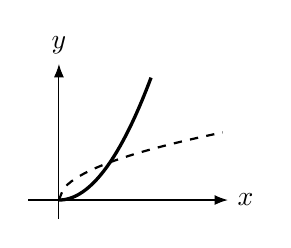
\begin{tikzpicture}[x=.65cm,y=.48cm,>=Latex]
\draw[->](-.6,0)--(3.3,0)node[right]{$x$};\draw[->](0,-.5)--(0,3.6)node[above]{$y$};
\draw[very thick,domain=0:1.8,samples=40]plot(\x,{\x*\x});
\draw[thick,dashed,domain=0:3.2,samples=40]plot(\x,{sqrt(\x)});
\end{tikzpicture}\par\footnotesize $x^2$ pro $x\ge0$ a jeho inverze $\sqrt{x}$
\end{minipage}\hfill
\begin{minipage}{.47\linewidth}\centering
\begin{tikzpicture}[x=.65cm,y=.48cm,>=Latex]
\draw[->](-2.2,0)--(3.35,0)node[right]{$x$};\draw[->](0,-3.6)--(0,3.6)node[above]{$y$};
\draw[very thick,domain=-1.8:0,samples=40]plot(\x,{\x*\x});
\draw[thick,dashed,domain=0:3.2,samples=40]plot(\x,{-sqrt(\x)});
\end{tikzpicture}\par\footnotesize $x^2$ pro $x\le0$ a jeho inverze $-\sqrt{x}$
\end{minipage}
\end{center}
\poznamka{Na pravém obrázku je vidět původní levá větev paraboly i její inverze v pravé dolní části soustavy. Pro kontrolu lze doplnit osu souměrnosti $y=x$; obrázek je pouze orientační výřez.}

\clearpage
\blok{Posunutá parabola}
\begin{prikladReseniBox}[title={Příklad 2}]
Funkce $g(x)=(x-1)^2+2$ je zadána na $D(g)=\langle1;+\infty)$. Urči $H(g)$, její inverzní předpis a ověř výsledek složením.
\tcblower
Na dané větvi je $g$ rostoucí a $H(g)=\langle2;+\infty)$.
\[
\begin{aligned}
g(x)&=(x-1)^2+2 &&\bigm|\ x\to y\\
x&=(y-1)^2+2\\
x-2&=(y-1)^2\\
y-1&=\sqrt{x-2}\\
y&=1+\sqrt{x-2}\\
g^{-1}(x)&=1+\sqrt{x-2}.
\end{aligned}
\]
$D(g^{-1})=\langle2;+\infty)$. Kontrola: $g^{-1}(g(x))=1+\sqrt{(x-1)^2}=1+|x-1|=x$ pro $x\ge1$.
\end{prikladReseniBox}

\begin{zadaniBox}[title={Věta - Složení inverzních funkcí}]
Pro prostou funkci $f$ a její inverzi platí
\[
f^{-1}(f(x))=x\quad (x\in D(f)),\qquad f(f^{-1}(y))=y\quad (y\in H(f)).
\]
\end{zadaniBox}
\noindent\textbf{Zdůvodnění.}\enspace Inverze po vykonání původního přiřazení vrátí výchozí argument. Původní funkce po vykonání inverze zase vrátí příslušnou funkční hodnotu; podmínky v závorkách zaručují smysluplnost obou složení.

\poznamka{Nepoužívej zápis $f(f^{-1}(x))=x$ bez připomenutí oboru $x\in H(f)$: právě zde vznikají chyby u druhé mocniny.}

\blok{Samostatná práce}
\begin{zadaniReseniBox}[title={Samostatná práce 1}]
\begin{enumerate}[label=\alph*)]
\item $f(x)=(x+2)^2$ pro $x\ge-2$: najdi inverzi a její definiční obor.
\item $g(x)=x^2$ pro $x\le0$: vypočítej $g^{-1}(25)$.
\item $h(x)=\sqrt{x-4}$ pro $x\ge4$: vypočítej $h^{-1}$ a zkontroluj $h^{-1}(h(13))$.
\end{enumerate}
\tcblower
\begin{enumerate}[label=\alph*)]
\item
\(\displaystyle\begin{aligned}f(x)&=(x+2)^2 &&\bigm|\ x\to y\\x&=(y+2)^2\\y+2&=\sqrt{x}\\y&=-2+\sqrt{x}\\f^{-1}(x)&=-2+\sqrt{x}\end{aligned}\)

$D(f^{-1})=\langle0;+\infty)$.
\item
\(\displaystyle\begin{aligned}g(x)&=x^2 &&\bigm|\ x\to y\\x&=y^2\\y&=-\sqrt{x}\\g^{-1}(x)&=-\sqrt{x}\end{aligned}\)

$g^{-1}(25)=-5$, protože původní argument splňuje $y\le0$.
\item
\(\displaystyle\begin{aligned}h(x)&=\sqrt{x-4} &&\bigm|\ x\to y\\x&=\sqrt{y-4}\\x^2&=y-4\\y&=x^2+4\\h^{-1}(x)&=x^2+4\end{aligned}\)

$D(h^{-1})=\langle0;+\infty)$ a $h^{-1}(h(13))=h^{-1}(3)=13$.
\end{enumerate}
\end{zadaniReseniBox}

\begin{zadaniReseniBox}[title={Rozšíření 1}]
Funkce $p(x)=(x-3)^2+1$ je zadaná na $(-\infty;3\rangle$. Urči inverzi a srovnej ji s případem $x\ge3$.
\tcblower
Pro levou větev $y\le3$:
\[
\begin{aligned}
p(x)&=(x-3)^2+1 &&\bigm|\ x\to y\\
x&=(y-3)^2+1\\
x-1&=(y-3)^2\\
y-3&=-\sqrt{x-1}\\
y&=3-\sqrt{x-1}\\
p^{-1}(x)&=3-\sqrt{x-1}.
\end{aligned}
\]
Pro pravou větev $y\ge3$:
\[
\begin{aligned}
p(x)&=(x-3)^2+1 &&\bigm|\ x\to y\\
x&=(y-3)^2+1\\
x-1&=(y-3)^2\\
y-3&=\sqrt{x-1}\\
y&=3+\sqrt{x-1}\\
p^{-1}(x)&=3+\sqrt{x-1}.
\end{aligned}
\]
V obou případech je $D(p^{-1})=\langle1;+\infty)$; obory hodnot se liší.
\end{zadaniReseniBox}

\begin{zadaniReseniBox}[title={Domácí úkol}]
\begin{enumerate}[label=\alph*)]
\item Urči inverzní funkci k $f(x)=(x+1)^2-3$ na $\langle-1;+\infty)$.
\item Vysvětli, proč $x^2$ na $\mathbb R$ inverzní funkci nemá, ale na $\langle0;+\infty)$ má.
\end{enumerate}
\tcblower
\begin{enumerate}[label=\alph*)]
\item
\[
\begin{aligned}
f(x)&=(x+1)^2-3 &&\bigm|\ x\to y\\
x&=(y+1)^2-3\\
x+3&=(y+1)^2\\
y+1&=\sqrt{x+3}\\
y&=-1+\sqrt{x+3}\\
f^{-1}(x)&=-1+\sqrt{x+3}.
\end{aligned}
\]
$D(f^{-1})=\langle-3;+\infty)$.
\item Na $\mathbb R$ mají opačné argumenty stejnou druhou mocninu; na nezáporné části je funkce prostá.
\end{enumerate}
\end{zadaniReseniBox}
\end{document}
